\section{Introduktion}

\begin{frame}{Data-Obliviousness}
	\begin{itemize}
		\item Hvad er Data-Obliviousness?

		\item Fordele
		\begin{itemize}
			\item Branches
			\item Hardware
			\item Parallisme
		\end{itemize}

		\item Ulemper
			\begin{itemize}
				\item Kompleksitet
		\end{itemize}
	\end{itemize}
\end{frame}

\begin{frame}{Data-Oblivious Sorting}
	\begin{itemize}
		\item Compare-Exchange
			\begin{itemize}
				\item Sæt 2 elementer i korrekt rækkefølge
			\end{itemize}
		\item \textcolor{red}{$\div$ Quicksort, Mergesort, Heapsort \dots}
		\item \textcolor{green}{$+$ Bitonic Sort, Pratt's Shellsort \dots}
	\end{itemize}
	\begin{block}{Compare-Exchange}
		\begin{algorithmic}
			\Procedure{Compare-Exchange}{$A, i, j$}
				\State $A_{min} \gets \min(A[i], A[j])$
				\State $A_{max} \gets \max(A[i], A[j])$
				\State $A[\min(i,j)] \gets A_{min}$
				\State $A[\max(i,j)] \gets A_{max}$
			\EndProcedure
		\end{algorithmic}
	\end{block}
\end{frame}

\begin{frame}{Deterministic Data-Oblivious Sorting Algorithms}
	\begin{columns}[T]
		\begin{column}{.48\textwidth}
			\begin{itemize}
				\item Sorteringsnetværk
				\item Long history
					\begin{itemize}
						\item Bitonic Sort (68)
						\item Odd-Even Mergesort (68)
						\item Pratt's Shellsort (72)
						\item AKS (83)
						\item Zig-Zag Sort (14)
					\end{itemize}
			\item Problematiske køretider
			\end{itemize}
		\end{column}
		\hfill
		\begin{column}{.48\textwidth}
			\begin{block}{8-Wire Bitonic Sort}
				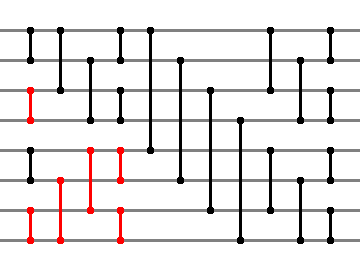
\includegraphics[width= \textwidth]{network.png}
			\end{block}
		\end{column}
	\end{columns}
\end{frame}

\begin{frame}{Randomized Data-Oblivious Sorting}
	\begin{itemize}
		\item Tilfældigt valgte sammenligninger
		\item Generelle algoritmer, dybde er ikke så vigtigt
		\item Nye algoritmer
			\begin{itemize}
				\item Randomized Shellsort (10)
				\item Annealing Sort (14)
			\end{itemize}
		\item Shaker Sort (87)
		\item Bedre køretider, ikke garanteret success
		\item Praktiske problemer
	\end{itemize}
\end{frame}


\begin{frame}<beamer:0>[noframenumbering]{Other Data-Oblivious Algorithms}
	\begin{itemize}
		\item Graf-algoritmer
		\begin{itemize}
			\item[] \mycite{ObliviousGraph}
		\end{itemize}
		\item Geometriske algoritmer
		\begin{itemize}
			\item[] \mycite{GraphGeoOblivious}
		\end{itemize}
		\item Mængde-Operationer
		\begin{itemize}
			\item[] \mycite{ObliviousSet}
		\end{itemize}
		\item En del flere \dots
	\end{itemize}
\end{frame}
